\documentclass{llncs}
\usepackage{enumerate}
\usepackage{amssymb,amsmath}
\usepackage{enumitem}
\usepackage{verbatim}


% xelatex
\usepackage{fontspec}
\usepackage{xunicode}
\usepackage{xltxtra}

%valodas. nez, vai vajag
\usepackage{polyglossia}
\setdefaultlanguage{english}
\setotherlanguages{latvian,russian}

% bibliography
%\usepackage{csquotes}
\usepackage[
    backend=biber,
    style=numeric-comp,
    sorting=none,
    natbib=true,
    url=false,
    doi=true%,
    %eprint=false
]{biblatex}
\addbibresource{bibliography.bib}


%images
\usepackage{graphicx}
\usepackage{float}

%dalīšana kolonnās
\usepackage{multicol}


\newcommand{\norm}[1]{\left\| #1 \right\|}

\begin{document}

\title{On the Hierarchy Classes of Finite Ultrametric automata}


\author{
Rihards Kri\v slauks, Kaspars Balodis}
\institute{University of Latvia Faculty of computing,\\ Rai\c na bulv\= aris 19, Riga, LV-1459, Latvia
}

\maketitle

\begin{abstract}
The work explores the language classes that arise with respect to the head count of a finite automaton. The results for deterministic non-deterministic and probabilistic automata are explored and similar results are proved for two-way ultrametric automata, which are viewed as a generalization of ultrametric finite automata that have just recently been introduced by ~\citet{Freivalds2012}. For the one-way setting it is shown that ultrametric one-head finite automata are more powerful than deterministic and non-deterministic automata for certain languages. Definitions for ultrametric Turing machines and ultrametric multi-register machines are introduced as a tool for proving the results. An interesting result regarding multi-tape automata is shown as well.
\end{abstract}



\section{Introduction} 
Ultrametric machines and Turing machines were first introduced by ~\citep{Freivalds2012}. This has been followed by several papers where various aspects of them are studied in depth. ~\citep{ KasparsBalodis2013} have studied the descriptional complexity of ultrametric automata. They show that ultrametric automata can achieve an exponential advantage in terms of the number of states required when compared to equivalent deterministic automata. ~\citep{Krislauks2013} have studied the reversal complexity of ultrametric Turing machines.

Ultrametric machines are similar to probabilistic machines, the difference being that it is not necessary for amplitudes (which are the equivalent of probabilities in probabilistic automata) to be in the range between 0 and 1. Instead arbitrary rational numbers can be used. We should note that in ~\citep{Turakainen1969} a similar generalization of probabillistic automata was introduced, where "probabilities" can be arbitrarily large numbers, and the acceptance criterion is whether the probability to be in an accepting state is greater than a given threshold, furthermore it was shown that this generalization is in fact equivalent to probabilistic automata. However, unlike in these pseudo-probabilistic machines, the definition of ultrametric machines uses the concept of a $p$-adic norm.

It can be said that the definition introduced by Freivalds is natural since it uncovers the only remaining notation %TODO pārfrāzēt
of a random variable not yet fully explored ~\citep{Freivalds2012}. In addition useful properties have been proven for the definition of ultrametric machines -- ~\citep{KasparsBalodis2013} proved that the language class recognized by regulated $p$-adic machines coincides with the class of regular languages.

In this paper most of the attention is given to the question of the language hierarchy associated with the head count of ultrametric multi-head automata. %TODO pārfrāzēt
Several results can be found in the literature which consider deterministic, nondeterministic and probabilistic finite automata in both -- the two-way and one-way -- cases ~\citep{Holzer2009, Yao1978, Monien1980, Macarie1995}. The paper examines whether similar results regarding the seperation in classes with respect to the head count can be achieved for ultrametric multi-head finite automata. Other results consider the relationships of the language classes recognized by ultrametric and classical automata.

\chapter{$p$-adic numbers}
\section{Introduction to $p$-adic numbers}
A $p$-adic digit is a natural number in the range of $0$ to $p-1$ (inclusive) where by $p$ we denote an arbitrary prime number. A $p$-adic natural number is a sequence %TODO varūt vajadzēja p-adic integers
$(a_i)_{i \in \mathbb{N}}$ where $a_i$ is a $p$-adic digit. This is the same as $\cdots a_i \cdots a_2a_1a_0$.
Which corresponds to a natural number given by
\[
\sum\limits_{i=0}^{+\infty}a_ip^i,
\]
where $p$ is our chosen prime number. This sequence is infinite to the left side. Furthermore - a natural number represented in $p$-adic numbers will have only a finite number of non-zero digits. For any given $n \in \mathbb{N}$ the non-zero part of its representation in $p$-adic numbers will exactly match $n$ representation in base $p$. Take the number $42$ as an example which is written as $123$ in base $5$. Its $5$-adic representation is $\cdots 0 \cdots 0132$.

The situation is different for negative and rational $p$-adic numbers. Take the number $\frac{1}{2}$ and its $5$-adic representation as an example. $5$-adic $\frac{1}{2}$ is a number which added to itself gives $1$. From this we can devise that the $5$-adic representation of $1$ is  
\[
\begin{tabular}{rrrrrrrrr|}
&$\cdots$ &2 &2 &2 &2 &2 &3\\
+&$\cdots$ &2 &2 &2 &2 &2 &3\\
\hline
\hline
&$\cdots$ &0 &0 &0 &0 &0 &1\\
\hline
\end{tabular}
\]

Similarly we devise subtraction and negative numbers. For example in $7$-adics
\[
\begin{tabular}{rrrrrrrrr|}
&$\cdots$ &0 &0 &0 &1 &3 &2\\
-&$\cdots$ &0 &0 &0 &2 &3 &4\\
\hline
\hline
&$\cdots$ &6 &6 &6 &3 &4 &3\\
\hline
\end{tabular}
\]
%Turklāt var ievērot, ka arī negatīviem skaitļiem informāciju satur tikai galīgs skaits ciparu pozīciju. Pozīcijās, kas ir pietiekami tālu pa kreisi atkārtojas cipars $p-1$.

Interestingly almost all rational numbers can be expressed in $p$-adics. The exceptions for a given $p$ are the numbers of the form $\frac{a}{b}$  where $a$ is not divisible by $p$ but $b$ is divisible by $p$.

Numbers that can't be expressed in $p$-adic natural numbers can however be expressed in $p$-adic rational numbers. Take the number $\frac{1}{5}$ as an example. It can't be expressed in $5$-dic natural numbers but it can be expressed as a $5$-adic rational number
\[
\cdots 0 \cdots 000,1.
\]
We can note that as with $p$-adic natural numbers $p$-adic rational numbers are expressed as a sequence which is infinite to the left side and finite to the right.

All of the usual arithmetic operations can be carried out on $p$-adic numbers as well, namely -- addition, subtraction, multiplication and division. Addition, subtraction and multiplication can be carried out in $p$-adic natural numbers %TODO šeit jābūt integers
but the results of subtraction can be general $p$-adic numbers.

It is obvious that for every $q \in \mathbb{Q}$ there exists a prime number $p$ such that $q$ can be expressed as a $p$-adic number. The same does not hold for real numbers. For every $p$ there exists an irrational number such that it cannot be expressed as a $p$-adic number. However that does not imply that for some $p$ $p$-adic numbers are a subset of real numbers. There is a continuum of $p$-adic numbers %TODO for every p?
that cannot be expressed as a real number ~\citep{Freivalds2012}.

\section{$p$-adic absolute values}
A function $d: X \times X \rightarrow R_{\geq 0}$ where $X$ is a non-empty set is called a metric iff it satisfies the following conditions:
\begin{enumerate}
\item $d(x,y) = 0$ iff $x = y$,
\item $d(x,y) = d(y,x)$,
\item $d(x,y) \leq d(x,z) + d(z,y)$ for all $z \in X$.
\end{enumerate}
The metric function is used to find the distances among the elements of a set. The distance of a given element to zero $d(x,0)$ is called the elements norm or absolute value and is denoted by $||x||$.

The norm satisfies the following properties
\begin{enumerate}
\item $||x||=0$ iff $x=0$,
\item $||x*y|| = ||x||*||y||$,
\item $||x+y|| \leq ||x||+||y||$ (triangle inequality).
\end{enumerate}
If the third property can be replaced with its stronger variant -- the strong triangle inequality %TODO apskatīties vai tā tulko
$||x+y|| \leq max(||x||,||y||)$ -- then the norm is said to be ultrametric. Otherwise it is called Archimedian ~\citep{Freivalds2012}.

\begin{definition}
For every non-zero rational number $\alpha$ there exists a unique prime factorization - $\alpha = \pm 2^{\alpha_2}3^{\alpha_3}5^{\alpha_5}7^{\alpha_7} \cdots$ where $\alpha_i$ are integers, only a finite number of which are non-zero.  The $p$-adic absolute value (also called the \textbf{$p$-norm}) of a rational number $\alpha$ is 
\[
||x||_p = \begin{cases}
p^{-\alpha_p}, &\textrm{if } \alpha \neq 0 \\
0, &\textrm{if } \alpha = 0.
\end{cases}
\]
\end{definition}

$p$-adic numbers in more detail are discussed in ~\citep{Madore}. The use of $p$-adics in other sciences can be seen in ~\citep{V.S.Vladimirov1995,Kozyrev2006,Dragovich2009}.

\chapter{One-way multi-head automata}
\section{Definitions}
Ultrametric automata are defined as in ~\citep{KasparsBalodis2013}.
\begin{definicija}
A finite $p$-ultrametric automata ($U_pFA$) is a sextuple %TODO 6-tuple?
$\langle S, \Sigma, s_0, \delta, F, \Lambda \rangle$ where
\begin{itemize}
  \item $S$ is a finite set -- the set of states,
  \item $\Sigma$ is a finite set ($\$ \notin \Sigma$) -- input alphabet,
  \item $s_0:S \rightarrow \mathbb{Q}_p$ is the initial amplitude distribution, %TODO vai tiešam pareizi?
  \item $\delta: \left( \Sigma \cup \left\{ \$ \right\} \right) \times S \times S \rightarrow \mathbb{Q}_p$ is the transition function,
  \item $F \subseteq S$ is the set of final states,
  \item $\Lambda = \left( \lambda, \diamond \right)$ is the acceptance condition where $\lambda \in \mathbb{R}$ is the acceptance threshold and $\diamond \in \left\{ \leq, \geq \right\}$.
\end{itemize}
The automaton works as follows.
At every timestep each of its states has an associated $p$-adic number called its amplitude.
The automaton starts with the initial amplitude distribution $s_0$.
Then it proceeds by processing input word's $w = w_1 \ldots w_n$ symbols one by one.
The amplitude distribution after processing the $i$-th symbol is denoted as $s_i$, with
$s_i(y) = \sum_{x \in S}{s_{i-1}(x) \cdot \delta \left( w_i, x, y \right) }$ for every $y \in S$.
After the $n$-th symbol, in the same way the end marker $\$$ is processed obtaining the final amplitude distribution $s_{n+1}$.
If the sum of the $p$-norms of final amplitudes over final states is at least (or at most) the threshold, i.e., if $\sum_{x \in F}{\left| s_{n+1}(x) \right|_p} \diamond \lambda$, then the word $w$ is said to be accepted, otherwise -- rejected.
\end{definition}

%TODO šo nevajag citā nodaļā?
A two-way $k$-head (where $k\geq 1$) finite autamaton consists of an input tape containing the input word on which the heads of the autamaton can move freely in both directions not crossing the endmarkers. The tape is read-only. More formally:
\begin{definition}[~\cite{Holzer2009}]
A non-deterministic $k$-head finite automaton ($2nfa(k)$) is a sextuple $\langle S, \Sigma, k, s_0, \delta, F \rangle$, where
\begin{itemize}
	\item $S$ a finite set -- the set of states,
	\item $\Sigma$ is a finite set ($ \triangleright,\triangleleft \notin \Sigma$) -- the input alphabet,
	\item $k\geq 1$ is the number of heads, 
	\item $s_0\in S$ is the starting state,
	\item $\delta: \left( \Sigma \cup \left\{ \triangleright, \triangleleft \right\} \right)^k \times S \times S \rightarrow \left\{-1,0,1\right\}^k$ is a transition function where $\triangleright$ and $\triangleleft$ are the start and end markers,
	\item $F \subseteq S$ is the set of accepting states.
\end{itemize}
\end{definition}
At the beginning of work a $2nfa(k)$ has all of its heads placed on the start marker. The automaton ends its work when the transition function $\delta$ is not defined for the current configuration. A configuration of a $2nfa(k)$ in some time moment $t\geq 0$ is a 3-tuple $c_t=\left(w,s,p\right)$ where $w$ is the input word, $s\in S$ is the current state and
$p = \left( p_1, \ldots, p_k \right) \in \left\{ 0, \ldots, |w| +1 \right\}^k $
gives the current head position. A transition from one configuration to the next is denoted by $\vdash$. A transition
$\left( w, s, \left( p_1, \ldots, p_k \right) \right) \vdash \left( w, s', \left( p_1+d_1, \ldots, p_k+d_k \right) \right)$
is valid iff
$\left(d_1, \ldots, d_k \right) \in \delta \left( \left( a_{p_1}, \ldots a_{p_k} \right) s, s' \right)$
where $w = a_1a_2 \ldots a_n$ is the input word and $a_0=\triangleright$ and $a_{n+1}=\triangleleft$. $\vdash$ reflexive transitive %TODO slēgums angliski
is denoted by $\vdash^*$.

The language $L(M)$ accepted by $M$ consists of those and only those words which are accepted by $M$. A $2nfa(k)$ accepts a word $w$ iff there exists a sequence of configurations that leads to automaton stopping in an accepting state if the input tape contains
$\triangleright w \triangleleft$. More precisely -- 
\begin{multline*}
	L(M)=\left\{ w \in \Sigma^* | \left(w,s_0,\left(1,\ldots,1\right)\right) \vdash^* \left(w,s,\left(p_1,\ldots,p_k\right)\right), s \in F,\right.\\
	\left.\textrm{un } M \textrm{ apstājas } \left(w,s,\left(p_1,\ldots,p_k\right)\right)\right\}.
\end{multline*}
If for any start state $\delta$ gives $\leq 1$ end state %TODO tā tulko izejas un izejas stāvokļus
then the automaton is said to be deterministic ($2dfa(k)$). If at any given moment the heads of an automaton move only right (or don't move) then the automaton is two-way. Nondeterministic and deterministic $k$-head automata are denoted by $1nfa(k)$ and $1dfa(k)$ respectively.
%TODO pabeigt par 2DFA(k). <-todo no bak darba


\section{Relation to classical automata}
Strictly inclusive classes have been shown for both one-way multi-head deterministic and nondeterministic automata with regard to the head count of the automata ~\citep{Holzer2009,Yao1978}. In 1978 ~\citet{Yao1978} showed that in order to separate the class of languages that can be recognized by a $1dfa(k)$ from that which can be recognized by a $1dfa(k+1)$ it is sufficient to use the language
\[
	L_n = \left\{w_1\$w_2\$ \ldots \$w_{2n} | w_i \in \left\{a,b\right\}^* \textrm{ un } w_i = w_{2n+1−i} \textrm{ visiem } 1 \leq i \leq n \right\}.
\]
We will consider a similar language -- $L_k$.
\begin{theorem}
For every $k \geq 1 \in \mathbb{N}$ there exists a language $L_k$ such that:
\begin{enumerate}[label={(\arabic*)}]
	\item for every $k \geq 1 \in \mathbb{N}$ there exists a $1u_pfa(1)$ that recognizes $L_k$,
	\item $L_k$ cannot be recognized by any $1dfa(k)$,
	\item $L_k$ cannot be recognized by any $1nfa(k)$.
\end{enumerate}
\end{theorem}
\begin{proof} The sought language is
\[
L_k = \left\{ w_1 1 w_2 1 \ldots 1 w_{2n} |
		w_i \in \left\{ 0 \right\}^m \wedge
		m \geq 1 \in \mathbb{N} \wedge
		w_i = w_{2n-i+1} \wedge
		n={k\choose 2}+1 \right\}.
\]
Now we prove that $L_k$ satisfies the points of our theorem.

$(1)$ We show that for an arbitrary language $L_k$ an $1u_pfa(1)$ can be built for every prime number $p$. The automaton starts its in $n$ different starting states $q_{1,1,1},q_{1,2,1},\ldots,q_{1,n,1}$ with amplitude $1$. Each of these states starts a "branch" that is intended for accumulating amplitude in one of $n$ different accepting states $q_{2n,1,2},q_{2n,2,2},\ldots,q_{2n,n,2}$. Every branch contains two kinds of states -- states of the 1st group $q_{i,j,1}$ are responsible for generating amplitudes and states of the 2nd group $q_{i,j,2}$ are intended for amplitude accumulation, $i \in \left[1, 2n \right], j \in \left[1, n \right]$.

If $0$ is read from the input and the automaton is in one of the 1st group states $q_{i,j,1}$ where $i \leq n$ then the amplitude of the state stays the same and with amplitude $1$ the automaton goes to a 2nd group state $q_{i,j,2}$. By doing so the states accumulated amplitude is added to $q_{i,j,2}$. If $0$ is read in a 2nd group state $q_{i,j,2}$ the states amplitude stays the same. If $1$ is read in a 1st group state $q_{i,j,1}$ where $i < n$ then the automaton with amplitude $j + 1$ transitions to $q_{i + 1,j,1}$ thereby transiting there with amplitude $(j + 1) \cdot \left| q_{i + 1,j,1} \right|$ (by $|q_i|$ we denote the amplitude the state $q_i$).
Whereas if $0$ is read in 1st group state $q_{i,j,1}$ where $i > n$ the amplitude of the state is kept unchanged and the transition to $q_{i,j,2}$ is made with amplitude $-1$. If $1$ is read in 1st group state $q_{i,j,1}$ where $i \geq n$ the transition to $q_{i + 1,j,1}$ is made with amplitude $-(j + 1)$. If $1$ is read in a 2nd group state a transition is made from $q_{i,j,1}$ to $q_{i + 1,j,1}$ with amplitude $1$. The exception is the last column of states -- $q_{2n,j,1}$ and $q_{2n,j,2}$ -- since they are responsible for reading in the last block of the word then the transition if $1$ is read is not defined. A schematic representation of the described automaton can be seen in \ref{fig:1pfa}.

\begin{figure}[h!]
\centering
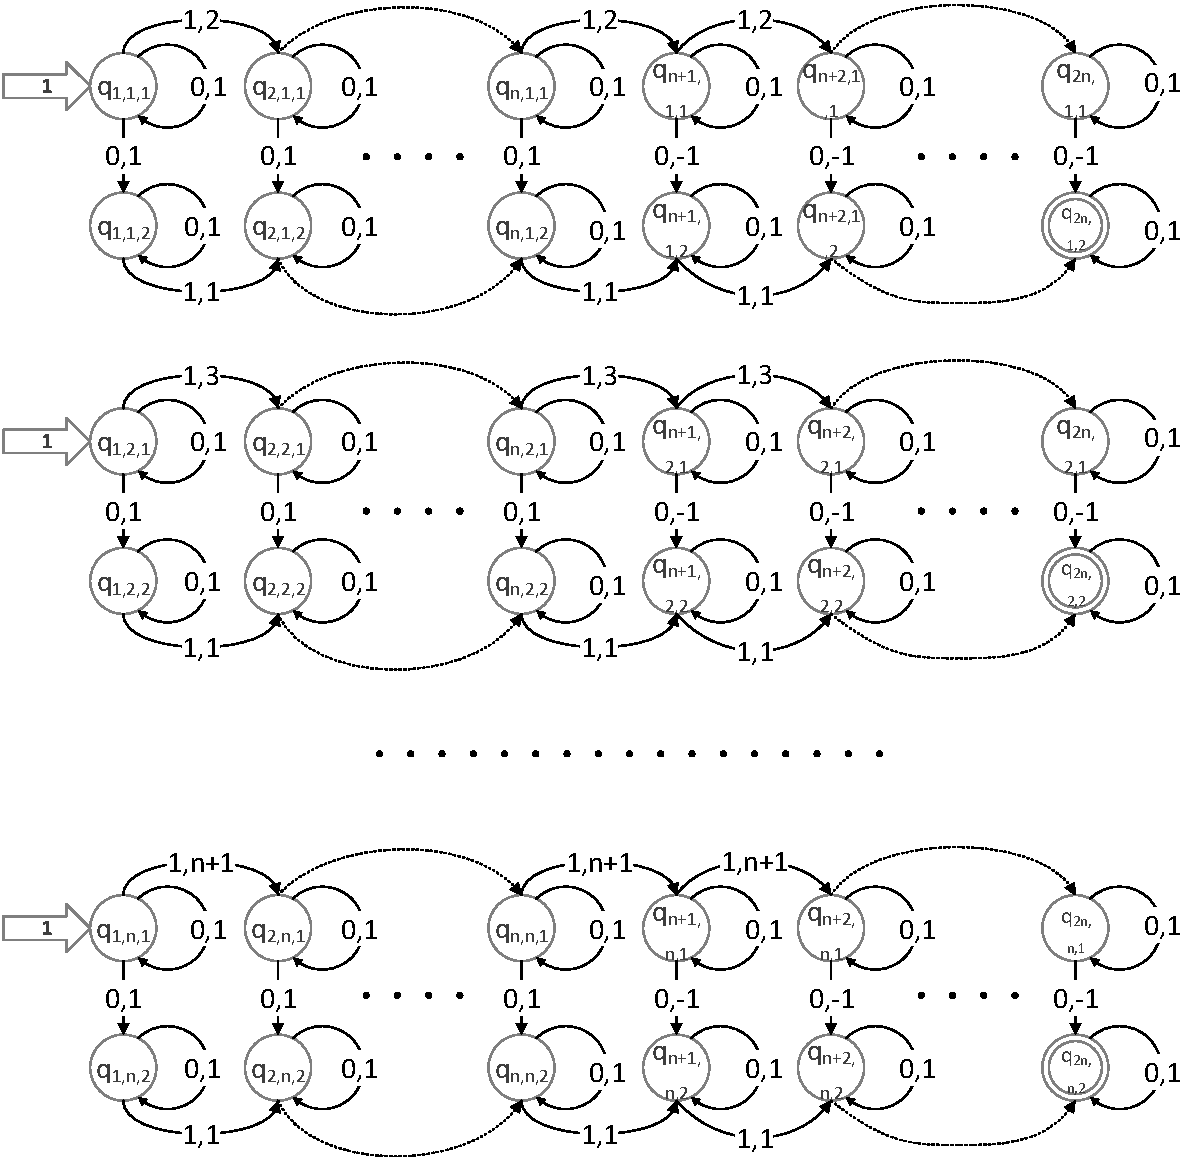
\includegraphics[width=\textwidth]{Img/1pfa.pdf}
\caption{Automaton to recognize $0^n10^m10^h1 \cdots 10^h10^m10^n$.}
\label{fig:1pfa}
\end{figure}

In result if a word $0^{a_1}10^{a_2}10^{a_3}1\ldots 10^{a_{2n}}$ was read then each of the accepting states $q_{2n,j,2}$ has accumulated an amplitude equal to
\[
	a_1 + a_2 \cdot (j + 1) + a_3 \cdot (j + 1)^2 + \cdots + a_n \cdot (j + 1)^{n - 1} - a_{n+1} \cdot (j + 1)^{n - 1} - a_{n+2} \cdot (j + 1)^{n - 2} - \cdots - a_{2n},
\]
which is equal to $0$ if the word belongs to the language; i.e. if
\[
	a_1 = a_{2n} \wedge a_2 = a_{2n-1} \wedge \ldots \wedge a_n = a_{n+1}.
\]
It follows that a word belongs to the language $L_k$ iff the following system holds:
\begin{gather*}
\allowdisplaybreaks
	\begin{cases}
		a_1 + a_2 \cdot 2 + a_3 \cdot 2^2 + \cdots + a_n \cdot 2^{n - 1} - a_{n+1} \cdot 2^{n - 1} - a_{n+2} \cdot 2^{n - 2} - \cdots - a_{2n} = 0 \\
		a_1 + a_2 \cdot 3 + a_3 \cdot 3^2 + \cdots + a_n \cdot 3^{n - 1} - a_{n+1} \cdot 3^{n - 1} - a_{n+2} \cdot 3^{n - 2} - \cdots - a_{2n} = 0\\
		a_1 + a_2 \cdot 4 + a_3 \cdot 4^2 + \cdots + a_n \cdot 4^{n - 1} - a_{n+1} \cdot 4^{n - 1} - a_{n+2} \cdot 4^{n - 2} - \cdots - a_{2n} = 0\\
		\cdots \\
		\begin{split}
		a_1 + a_2 \cdot (n + 1) + a_3 \cdot (n + 1)^2 + \cdots + a_n \cdot (n + 1)^{n - 1} - a_{n+1} \cdot (n + 1)^{n - 1} \\
		\qquad- a_{n+2} \cdot (n + 1)^{n - 2} - \cdots - a_{2n} = 0\\
		\end{split}
	\end{cases}\\
\intertext{rewriting}
	\begin{cases}
		(a_1 - a_{2n}) + 2 \cdot (a_2 - a_{2n-1}) + 2^2 \cdot (a_3 - a_{2n-2}) + \cdots + 2^{n - 1} \cdot (a_n - a_{n+1}) = 0\\
		(a_1 - a_{2n}) + 3 \cdot (a_2 - a_{2n-1}) + 3^2 \cdot (a_3 - a_{2n-2}) + \cdots + 3^{n - 1} \cdot (a_n - a_{n+1}) = 0\\
		(a_1 - a_{2n}) + 4 \cdot (a_2 - a_{2n-1}) + 4^2 \cdot (a_3 - a_{2n-2}) + \cdots + 4^{n - 1} \cdot (a_n - a_{n+1}) = 0\\
		\cdots \\
		\begin{split}
		(a_1 - a_{2n}) + (n + 1) \cdot (a_2 - a_{2n-1}) + (n + 1)^2 \cdot (a_3 - a_{2n-2}) + \cdots \\
		\qquad+ (n + 1)^{n - 1} \cdot (a_n - a_{n+1}) = 0\\
		\end{split}	
	\end{cases}
\end{gather*}

We see that the coefficients of the system form a Vandermonde matrix therefore its determinant is non-zero and since the given system is homogeneous only the trivial solution exists.

However if the word does not belong to $L_k$ then some no more than $4$ lines can hold true but even then there will be atleast one line which is not equal to $0$. %(citādi būtu nenulles risinājums, un sistēmai būtu netriviāls atrisinājums)
Therefore we can choose $0$ as a threshold for the acceptance condition -- we say that a word belongs to $L_k$ iff the accepting state end amplitude norm sum is $\leq 0$ and it does not belong to the language if contrary.

$(2)$ Proven by ~\citet{Freivalds1982} ~\citep{Freivalds1979} a proof for a similar language can also be found in ~\citep{Yao1978}. The idea of the proof relies on the fact that, any two heads that have been used to compare a pair cannot be used to compare another pair. This implies that if the number of block pairs in a word $n$ is greater than the number of pairs of heads ${k\choose 2}$ then the language cannot be recognized with $k$ heads.

$(3)$ Proven by ~\citet{Freivalds1982} a proof for a similar language can be found in ~\citep{Yao1978}.
\end{proof}

%TODO nākamais lieki tērē vietu?
It should be noted that to recognize $L_k$ a constant number of heads is enough for a probabilistic automaton as well. ~\citet{Freivalds1982} has prooved that for every $\epsilon > 0$ there exists a $1pfa$ that accepts every word in $L_k$ with probability $1$ and rejects others with probability $1 - \epsilon$.

\chapter{One-way multi-head automata}
%TODO

\chapter{Two-way automata}
\section{Definitions}
Ultrametric multi-head automata are defined by generalizing ~\citep{KasparsBalodis2013} definition of ultrametric automata in a most natural way. The definition of multi-head automata due by ~\citep{Holzer2009} is used as well.

\begin{definition}
A finite $k$-head two-way $p$-ultrametric automaton ($2u_pfa(k)$) is a 7-tuple $\langle S, \Sigma, k, s_0, \delta, F, \Lambda \rangle$ where
\begin{itemize}
	\item $S$ a finite set of states,
	\item $\Sigma$ a finite set ($ \triangleright,\triangleleft \notin \Sigma$) -- input alphabet,
	\item $k\geq 1$ the number of heads, 
	\item $s_0:S \rightarrow \mathbb{Q}_p$ the initial distribution of amplitudes,
	\item $\delta: \left( \Sigma \cup \left\{ \triangleright, \triangleleft \right\} \right)^k \times S \times S \rightarrow \mathbb{Q}_p \times \left\{-1,0,1\right\}^k$ the transition function where $\triangleright$ and $\triangleleft$ are the start and end markers,
	\item $F \subseteq S$ is the set if accepting states,
	\item $\Lambda = \left( \lambda, \diamond \right)$ the acceptance condition where $\lambda \in \mathbb{R}$ is the acceptance threshold $\diamond \in \left\{ \leq, \geq \right\}$.
\end{itemize}
\end{definition}

$2u_pfa(k)$ works in a similar way than $u_pfa$ with the exception that the automaton now has $k$ heads which can move freely similarly as in a $2nfa(k)$. In difference from a $u_pfa$ now amplitudes are given for a pair consisting of the positions of the heads and a state. The amplitude of the state $y \in S$ with heads in positions
$\left( p_1, \ldots, p_k \right) \in \left\{ 0, \ldots, |w| +1 \right\}^k $
after the $i$-th operation is given by
\[
s_i (y, (p_1, \ldots, p_k)) =
\sum_{\mathclap{\substack{ x \in S \wedge \\
		\exists (p'_1, \ldots, p'_k):
		(p'_1, \ldots, p'_k) +
		\delta ((w_{p'_1}, \ldots, w_{p'_k}), x, y)_2 =
		(p_1, \ldots, p_k)}}}
	{s_{i-1}(x) \cdot \delta ((w_{p'_1}, \ldots, w_{p'_k}), x, y)_1 }
\].

Similarly than before the acceptance condition is applied to the final amplitude $p$-norm sum of the accepting states. That is, if
\[
\sum_{\mathclap{\substack{x \in F \wedge\\
		\exists (p_1, \ldots, p_k):
		\textrm{ automāts beidz darbu stāvoklī } x
		\textrm{ ar galviņām pozicijās } (p_1, \ldots, p_k) }}}
	{\left| s_{n+1}(x, (p_1, \ldots, p_k)) \right|_p} \diamond \lambda
\]
then we say that $w$ belongs to the language and it doesn't if contrary.

Ultrametric Turing machines are defined to be used as a device to help prove results regarding multi-head automata classes. The basis for the definition is a definition for Turing machine by J. Hopcroft un J. Ullman ~\citep{Hopcroft1979} 1979. Well define a multi-tape Turing machine.
\begin{definition}
A $p$-ultrametric turing machine with $k$ work tapes $(U_pTM(k))$ is a 7-tuple $M= \langle Q, \Sigma, b, \Sigma, \delta, q_0, F \rangle$ where:
\begin{itemize}
	\item $Q$ is a nonemty set of states,
	\item $\Sigma$ is a nonempty set -- the working alphabet,
	\item $b \in \Sigma$ the "empty" symbol,
	\item $\Sigma\subseteq\Sigma\setminus\{b\}$ the input alphabet,
	\item $q_0 \in Q_p$ is the initial amplitude distribution,
	\item $F \subseteq Q$ is the accepting state set,
	\item $\delta: Q \setminus F \times \Sigma^k \rightarrow Q \times \left(\Sigma \times \{L,N,R\} \times \mathbb{Q}_p \right)^k$ is a partly defined transition function where $L$ denotes moving the head to the left, $R$ -- to the right and $N$ -- not moving the head and $\mathbb{Q}_p$ is the amplitude with which the transition is made.
\end{itemize}
\end{definition}

Similarly than with ultrametric multi-head automata the machine with a given amplitude is in one of its possible configurations. However now the configuration consists of state of the logic block %TODO noteikti jānoskaidro, kā tulkojas vadības bloks
and the contents of all $k$ tapes. The amplitude with which the machine is in one of its configurations in the $i$-th step is computed analogously than in the case with ultrametric multi-head automata. From now on when saying that a Turing machine accepts a word we mean that the machine stops in an accepting state after it is done processing the word as input. The criteria for acceptance are analogous to those of ultrametric multi-head automata.
%(jāievēro tikai, ka tagad automāta konfigurācijā ietilpst arī no lentes saturs, un amplitūda tiek piekārtota tam kombinācijā ar vadības bloka stāvokli).

Ultrametric multi-register automata are also used as an intermediate device for proofs.
\begin{definition}
A finite $p$-ultrametric $k$ register automaton (also machine) ($2u_pra(k)$) consists of a $p$-uptrametric logic block and $k$ registers that can hold natural numbers. The automaton begins with the input word in the first register and according to the specified amplitude distribution in some of its states. A predicate $\stackrel{?}{=} 0$ and the operations $+1$ or $-1$ can be applied to a register. Each of the transitions of the logic block can have a predicate or an operation associated with it which is triggered when the transition is made. Acceptance criteria are analogous to those of ultrametric automata.
\end{definition}
\printbibliography
